%%%%%%%%%%%%%%%%%%%%%%%%%%%%%%%%%%%%%%%%%%%%%%%%%%%%%%%%%%%%%%%%%%%%%%%%%%%%%%%%%%%%%%%%%%%%%%%%%%%%%%%%%%%%%%%%%%%%%%%%%%%%%%%%%%%%%
\section{Notations and Conventions}
\label{sec:definitions}

This section presents the notations and definitions used in this work. Define the infinite set $\mathbb{\bar{N}}_1 = \{ \bar{1}\,, \bar{2}\,, \hdots \}$. Unless otherwise stated, $i, j, k \in \mathbb{N}_0 \cup \mathbb{\bar{N}}_1 \cup \{b,\bar{b},e\}$.
%
\begin{figure}[ht]
    \centering
    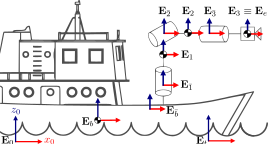
\includegraphics[width=1\columnwidth]{figs/ship_conventions.pdf}
    \caption{Frame conventions for the 3 DOF ISP system installed on a vessel.}
    \label{fig:HEADS_convention}
\end{figure}

Considering \fref{fig:HEADS_convention}, define the following coordinate frames, matrices, vectors and scalars:
%
\begin{itemize}
\item $\mathbf{E}_0$: inertial frame, arbitrarily positioned;
\item $\mathbf{E}_{\bar{b}}$: vehicle frame placed anywhere on the vehicle;
\item $\mathbf{E}_b$: vehicle frame located on its center of mass (CM);
\item $\mathbf{E}_{\bar{i}}$: fixed on link $i$ with origin on joint $i$ axis $(i \in \mathbb{N}_1)$;
\item $\mathbf{E}_{i}$: fixed on link $i$ with origin on its CM ($i \in \mathbb{N}_1$);
\item $\mathbf{E}_{e}$: end-effector frame;
\item $\mathbf{E}_{t}$: fixed on the target georeferenced position;
\item $R_{ij} \in SO(3)$: rotation matrix describing the orientation of frame $\mathbf{E}_j$ relative to frame        $\mathbf{E}_i$;
%Of course, $R_{i,i} = I_{3}$, where $I_{3} \in \mathbb{R}^{3 \times 3}$ is the identity matrix;
%
\item $x^k_i\,,y^k_i\,,z^k_i \in \mathbb{R}^{3}$ are the canonical unit vectors of $\mathbf{E}_i$, expressed in $\mathbf{E}_k$;
%
%\item $p_{0i} \in \mathbb{R}^{3}$: inertial position of the origin of frame $\mathbf{E}_i$;
%
\item $r^{k}_{ij} \in \mathbb{R}^{3}$: vector from the origin of frame $\mathbf{E}_i$ to the origin of $\mathbf{E}_{j}$, represented in $\mathbf{E}_k$. We use $r=p$ for position and $r=v$ for linear velocity, for example;
%
\item $g_{ij} \in SE(3)$: homogeneous transformation matrix from frame $\mathbf{E}_j$ to frame $\mathbf{E}_i$;
%depending on $R_{ij}$ and on the position vector $p^i_{ij}$;
%
%\item $h^{j}_{i} \in \mathbb{R}^{3}$: unit vector defining the rotation axis of joint $i$, represented in $\mathbf{E}_j$ ($i \in \mathbb{N}_1$);
%\item $\omega_i \in \mathbb{R}^{3}$: angular velocity of body $i$ seen and represented in the inertial frame 					 $\mathbf{E}_0$ ($i \in \mathbb{N}_1 \cup \{b\}$). Mathematically, $\omega_i$ is defined as the twist coordinates of the $so(3)$ 			 Lie algebra as $\hat{\omega}_i = \dot{R}_i R^{T}_{i}$;
%
\item $m_i \in \mathbb{R} ,\, I^i_i \in \mathbb{R}^{3 \times 3}$: mass and inertia matrix of body $i$ represented in its  local frame
$\mathbf{E}_{i}$ ($i \in \mathbb{N}_1 \cup \{b\}$);
%
\item $\overline{I}^i_i =
\left[\begin{array}{cc}
\!\! m_i \, I_{3\times3} \!\!&\!\!  0 \!\! \\
\!\! 0 \!\!&\!\! I^i_i \!\!
\end{array}\right]$: augmented inertia matrix of body $i$.
%of body $i$ written in $\mathbf{E}_{i} (i \in \mathbb{N}_1 \cup \{b\})$.
%
\end{itemize}

In this work, if the superscript symbol is omitted, the vector is represented in $\mathbf{E}_0$.
%
Note that, by the definition of $\mathbf{E}_{i}$, $I^i_i$ is a constant matrix. If $\mathbf{E}_{i}$ is chosen to be aligned with the principal axis of inertia of rigid body $i$, $I^i_i$ is also diagonal.   Therefore,
for simplicity, it is supposed that the principal moments of the inertia matrix of body $i$ are known.
%
Also, in the case of a 3 DOF ISP, we suppose that $\mathbf{E}_{e} \equiv \mathbf{E}_{3}$.
